%
\documentclass[Journal]{ascelike}
%
% Feb. 14, 2013
%
% Some useful packages...
%
\usepackage{manyeqns}
\usepackage{graphicx}
%\usepackage{subfigure}
\usepackage{amsmath}
\usepackage{amsfonts}
\usepackage{amssymb}
%\usepackage{amsbsy}
%\usepackage{times}
\usepackage{color}
\usepackage{listings}
%
% Place hyperlinks within the pdf file (works only with pdflatex, not latex)
% \usepackage[colorlinks=true,citecolor=red,linkcolor=black]{hyperref}
%
%
% NOTE: Don't include the \NameTag{<your name>} if you have selected 
%       the NoPageNumbers option: this leads to an inconsistency and
%       a warning, and the NameTag is ignored.
%\NameTag{Nam Lethanh, April. 02, 2014}
%
%
\begin{document}
%% You will need to make the title all-caps
\title{Prediction of Road Section Condition with Incomplete Inspection Data using a Longitudinal Univariate Kriging 
Model}%
\author{
Nam Lethanh \thanks{Research Associate, Dr., Institute of Construction and Infrastructure Management., Swiss Federal 
Institute of Technology (ETH), 8093 Zurich, Switzerland. E-mail: lethanh@ibi.baug.ethz.ch}, Craig Richmond 
\thanks{Research Associate, Dr., Institute of Construction and Infrastructure Management., Swiss Federal 
Institute of Technology (ETH), 8093 Zurich, Switzerland. E-mail: richmond@ibi.baug.ethz.ch} and Bryan T. Adey%
\thanks{Asso. Prof, Dr., Institute of Construction and Infrastructure Management., Swiss Federal 
Institute of Technology (ETH), 8093 Zurich, Switzerland. E-mail: adey@ibi.baug.ethz.ch}\
}
%
\maketitle
%
\begin{abstract}
A longitudinal univariate Kriging model is formulated and tested on a set of serviceability indicators for the Swiss 
national highway network. The predictive power of the model is then investigated across various formulations of the 
model and across serviceability indicators for surface defects, longitudinal and transversal evenness. Such a model can be used to predict values of the indicators at locations where no measurements were recorded. Unfortunately, that is a common problem when working with more than one independent set of GIS indexed data because the data is frequently recorded for non-coincidental GIS shapes. It is shown that the model is feasible and can be used as a predictive instrument for missing values with reasonably high levels of accuracy. The predictive ability varies not only by formulation but also by indicator and even by inspection campaign. Thus, in a practical application, the model’s specification should be adjusted to best fit the characteristics of the data using a procedure such as the one as outlined here.
\end{abstract}
%
% Some keywords, using a new command: \KeyWords{}
%
\KeyWords{Kriging method; Pavement management; Optimal intervention strategy; Deterioration prediction.}
%
\section{Introduction} \label{introduction}
Roads, obviously, are longitudinally connected and this is equally true of measures of physical conditions along the 
road; they will also be longitudinally connected in the sense that two measurements along the road will be spatially 
correlated if the measurements are sufficiently close to one another. This fact provides the basis of a strategy to 
predict values where such are missing. ‘Missing’ values occur more frequently than one would expect for the simple 
correlated if the measurements are sufficiently close to one another. This fact provides the basis of a strategy to predict values where such are missing. ‘Missing’ values occur more frequently than one would expect for the simple reason that the physical condition of the road varies continuously whereas recorded observations are normally discreet. Occasionally, of course values from an inspection campaign are truly missing, in the sense that a panel data set has an empty cell. But that is not the only need for a means to interpolate values in between those that are known. A second case arises even when all intended data sets are complete but when they are referenced with two independent GIS shape file, for example if measures of longitudinal unevenness referenced to road segments are to be matched to GIS indexed soil type data. The former may be recorded every 100 $m$ along the road while the other may be recorded on a completely unrelated 100 $m^2$ raster. The two shapes will normally not have coincident boundaries making it fundamentally uncertain which values should be connected to which in the overlapping regions. This second case is endemic to working with GIS data sets. Thus, even if no values are truly missing, from an operational point of view, one still may not have observations everywhere where they are needed. 

In such cases, one must make some assumption on how to relate the two data sets. One possibility is to estimate the missing value using a distance weighted average of the overlapped observations from the first set of measurements and then relate those to the second set of measurements. However, that ad-hoc procedure may not be the best way to predict an intermediate value. An alternative means is to treat the overlapped areas as separate ``missing'' observations and estimate them explicitly from nearby observations. One method for doing that is Kriging. 

Kriging models originated in the field of geostatistics, but are now used in several engineering fields 
\cite{Wackernagel1998}. The principle of Kriging is to estimate the missing value at a target point from optimally 
derived weights applied to observations at nearby points. The predicted target value is then calculated as a linear combination of the 
observed values. Importantly, the weights depend both on the spatial correlation and on the spatial distribution of the 
points. This paper begins with an investigation of the spatial correlation of the road serviceability indicators in a 
data set on the Swiss national highway network. Interestingly the spatial correlation varies by indicator and even for 
the same indicator, by the inspection campaign. A study of spatial correlation is interesting in its own right and 
three potential additional uses of spatial correlation beyond the prediction of missing values are:

\begin{itemize}
 \item to determine the optimal distance between inspections
 \item to evaluate different inspection technologies
 \item to identify potential measurement or data entry errors through a comparison with kriged values
\end{itemize}
%
No methods to exploit such opportunities are presented here, but the potential uses do make the investigation of spatial 
correlation more meaningful.

The remaining paper is structured as follows. Following section presents a literature review on techniques and methods used for estimating missing data, especially in the context of infrastructure systems. Section \ref{spatialcorrelation} gives an overview of the derivation of the variograms, which express the spatial correlation relationships. Section \ref{krigmodel} introduces a general formulation of Kriging models. Section \ref{krigestimate} presents the estimation methodology to be applied here. Section \ref{casestudy} reports the results of an application to data from the Swiss national highway network. The last section includes the conclusions and potential research extensions.

\section{A review on missing data estimation} \label{missingdata}
\textcolor{red}{One of the good review works on the estimation of missing data, especially in the context of infrastructure management systems, is the work of \citeN{AlZoubi2015}. The cited work summarises a the development of methods and techniques used to populate missing data over the last decades in different fields of studies using statistical analysis of data. The cited authors also recommended a so-called ``systematic statistical approach (SSA)'' to populate the missing data in the pavement management system (PMS). This is therefore, this section does not attempt to restate the literature review concerning the treatment for missing data or how to reestimate missing data. For understanding deeper on this subject, it is advisable to refer to the cited paper and other literatures on the fields of statistica analysis \cite{Little2002,Tsikriktsis2005}. In this section, it is important to highlight some prominent works in the PMS and discuss the SAA, which is considered as the first research work for reestimating missing data in the PMS.}

\textcolor{red}{According to the \citeN{AlZoubi2015}, in the domain of pavement management research, there has been no coverage on which methods and approaches used to reestimate the missing data. To the best of the authors knowledge, this statement of the cited authors was true. It does not infer that the problem of missing data is not covered. In fact, many research works have considered missing data, censorred data, truncated data, and measurement errors in the estimation process for obtaining the most likely values of models' parameters. For example, \citeN{Ben-Akiva1993,Ben-Akiva1995} proposed an statistic approach to predict latent deterioration of infrastructure objects. Later, \citeN{Chu2008} suggested the use of an AutoRegressive Integrated Moving Average model and Kalman filter to deal with panel data sets containing missing data. Solving for the model's parameters given incomplete or hetegernous data sets became more versatile and robust when Bayesian estimation approach was introduced \cite{Hong2006,Kobayashi2012a,Lethanh2015b}.}

\textcolor{red}{In order to reestimate the missing data, two basic techniques can be employed. The first technique is to use the ``model-free replacement technique (MFRT)'' and the second one is ``model-based replacement technique (MBRT) \cite{AlZoubi2015}. The MFRT does not require any mathematical model to reestimate the missing data, rather it relies on simple interpolation techniques. For example, if data of road section is missing, engineer might use the values of serviceability indicators in nearby sections and take the mean values or use the moving average (reestimating missing value with the last available data point) \cite{AlZoubi2015}. This ad-hoc reestimation technique, as mentioned earlier in the introduction section, could bear bias and might not be the best way to predict missing value. With the MBRT, it is required to define a time or paremeter dependent function of the serviceability indicators. Example of such function is the $sigmoidal$ function used by the Texas Department of Transportation \cite{Stampley1995} and the exponential function used to capture the evolution of international roughness index over time \cite{paterson90}. Values of parameters in the pre-defined functions in the MBRT are estimated from available data by means of various regression techniques (e.g. linear regression, cubic regression, cubic spline based on nearby serviceability indicators) \cite{AlZoubi2015}. After values of model's parameters are obtained, the value of a serviceability indicator, which is missing, can be straitforward computed. }

\textcolor{red}{The work of \citeN{AlZoubi2015} has laid one of the first stones on the problem of populating missing data in the PMS. However, it has following limitations:}

\textcolor{red}{\begin{itemize}
 \item It did not perfectly consider the spatial correlation despite the fact that it mentioned simple interpolation techniques based on values of serviceability indicators in nearby locations. In other words, the distance was ruled out. The authors only looked into the physical records in the database but not consider the spatial correlation. For example, in the case study of the cited paper, the authors used the mean and median of nearby points. However, the distance between two adjacent points are neary 1 km long. With such a long distance, it is likely to have a week correlation on their values.
 \item It only looked into the true missing data but but not oversaw another types of missing data that is derived from managerial perspectives. Example of this type of missing data is data that managers expect to obtain from GIS records, which was explicitly mentioned in the introduction section. For example, there are two sets of data collected from two consecutive inspection campaigns and these two data sets have no missing data. However, they were not recorded in exact the same ways, resulting in overlapping of sections, even in a very small distance. 
 \item The proposed SSA can be used for obtaining the true missing value in the database, but it cannot be used for determination of optimal inspection distance since the spatial correlation is not included. Furthermore, techniques used in the SSA are univariate. This means, it is not possible to use the value of one serviceability indicator to estimate the value of the other one. 
\end{itemize}}
\section{Spatial correlation of serviceability indicators of roads} \label{spatialcorrelation}
In Switzerland, there are six road serviceability indicators. Our data however only contained observations for three 
of them: $I0$, $I2$, and $I3$. Their definitions are given in Table \ref{table1}. These indicators are continuous 
within the range $[0,5]$ where the best state is zero. Detailed standards exist on their measurement\footnote{VSS Norm 640925b governs the current assessment of I-Values in Switzerland.} and yet achieving comparable measurements across inspection campaigns is not a trivial matter. This is particularly true for $I0$ that 
involves a visual assessment of the severity and extent of the damage to the road’s surface. 
%%
\begin{table}
\begin{center}
\caption{Definition of inspection values.}
\label{table1}
\begin{tabular}{c|l}\hline
\textbf{I values} & \textbf{Description}\\\hline
I0 & is used to describe the surface damage without consideration of rut index\\
I1 & is used to describe the surface damage with consideration of rut index\\
I2 & is used to describe the longitudinal unevenness\\
I3 & is used to describe the transversal unevenness\\
I4 & is used to describe the surface friction\\
I5 & is used to describe the load bearing capacity\\\hline
\end{tabular}
\end{center}
\end{table}
%%

Indicator observations can be gathered either manually, where a person physically inspects the road, or by means of an 
automated inspection vehicle that drives over the road and records measurements of the indicators as it passes. In some 
cases videos are made for separate manual evaluation. The data is then stored in a database to be used, for instance, in 
planning interventions. The distance between observations, and hence the number of observations, has an impact on the 
cost of the inspection campaign as well as on the number of records in the database. The intervals may be as short as 
$100$ $m$ or as long as $1000$ $m$. In the case of automated inspection cars, the underlying observations may in fact be continuous even if the records in the database are average values over the whole section length. Thus the question of optimal inspection interval cannot be answered in the abstract, but depends on the cost per observation and the degree of spatial correlation. If spatial correlation is high, then intervals can be longer, all else equal.

Fig. \ref{fig1} shows the spatial correlation of serviceability indicators for the Swiss national highway network. The 
inspection campaign in the year 2000 did not include an observation for $I0$. The 2004 and 2009 campaigns measured all three indicators. One sees that the lowest correlation values for both $I2$ and $I3$ occur in 2000. Barring these two observations, which probably reflect a less accurate inspection method, there is a rank order in spatial correlation where $I0 > I3 > I2$. That is, longitudinal unevenness, $I2$, appears to have the most spatial randomness and surface defects, $I0$, the most spatial correlation. The reader should note that the values calculated at zero meters difference are deceptive since in fact, there is only one measurement at each point and the correlation with itself must be 1. If two independent inspections were executed at the same place, it is unlikely that the correlation would be 1. The evidence of spatial correlation declining in distance is nonetheless strong. One also notes that the rate of decline levels off in all three cases after about $400$ $m$ and it remains clearly above zero even at $1000$ $m$ difference. Considering that the length of a typical intervention on a national highway is likely to be longer than $1000$ $m$, this result is to be expected due to shared histories of construction, maintenance and use. An alternative, but not mutually exclusive cause, might be forward propagation of damage through the induced motion on passing vehicles.
%
\begin{figure}
\centering
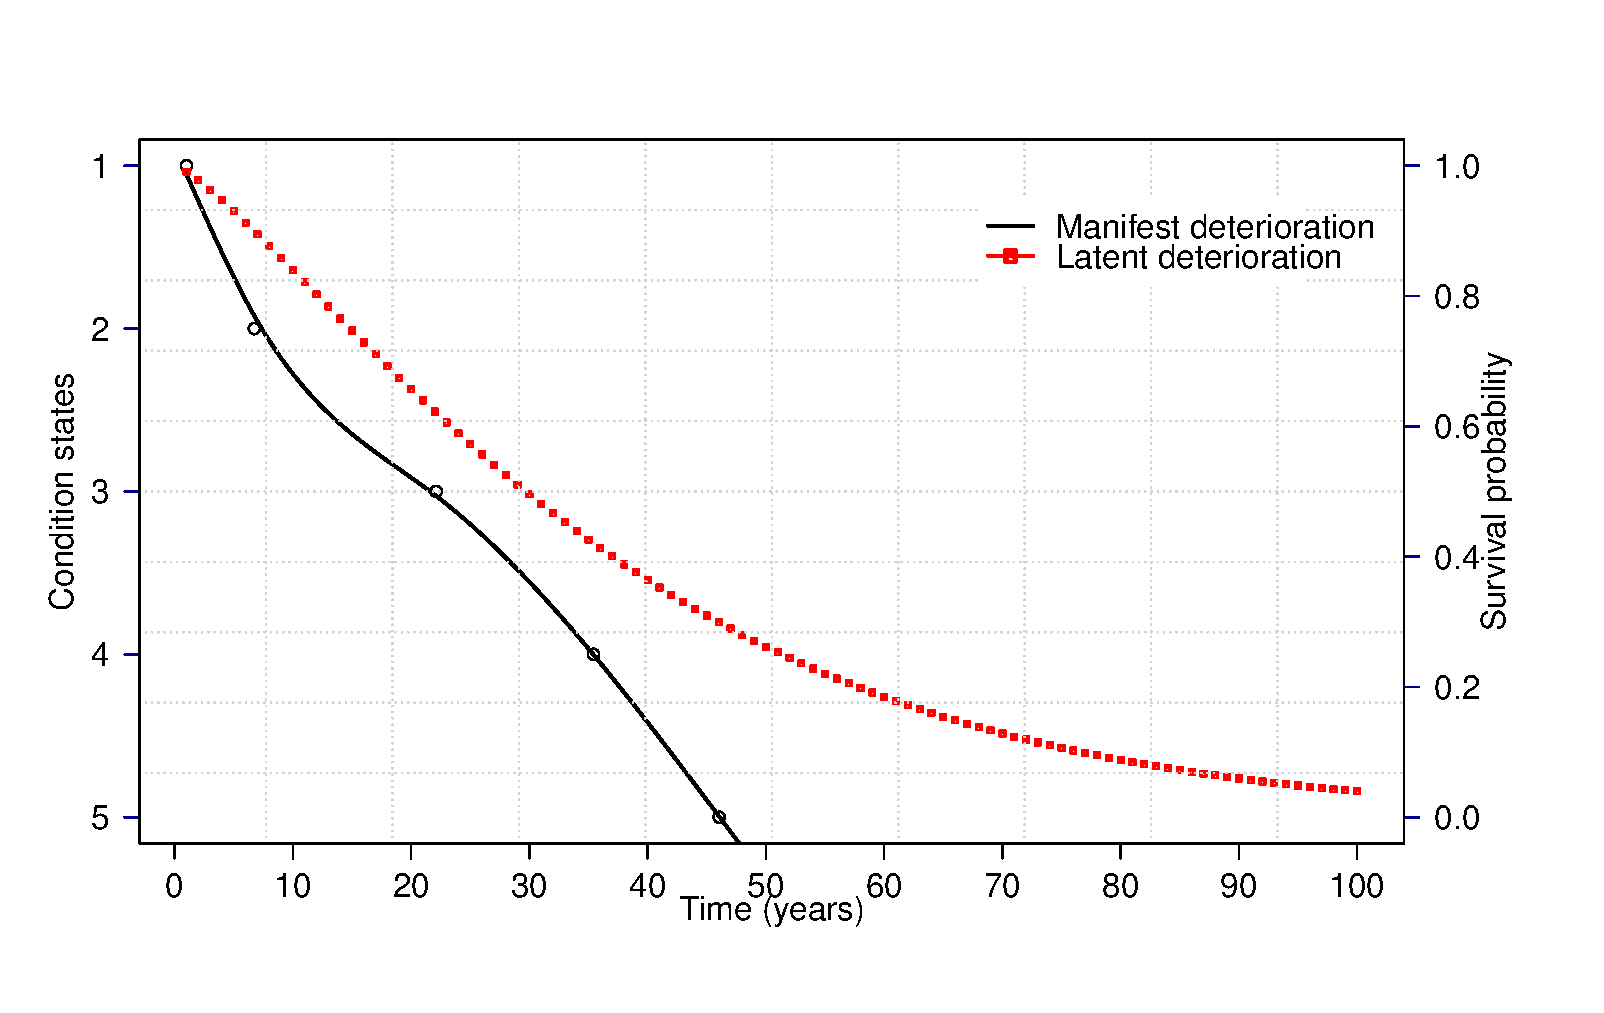
\includegraphics[scale=0.6]{fig1} 
\caption{Spatial correlation of serviceability indicators.} 
\label{fig1}
\end{figure}
%
Spatial correlation is expressed in Kriging models through a theoretical variogram which is defined in Eq. (\ref{varab1}). It 
expresses the functional relationship between distance and the variance of the difference between two random variables. 
Using the definitions of variance, covariance and correlation one can express the relationship between the two random 
variables as follows
%%
\begin{eqnarray}
&& Var(a-b)=\sigma_a^2+\sigma_b^2-2\sigma_a\sigma_b\rho_{a,b}\label{varab1}
\end{eqnarray}
%%
\textcolor{red}{Where, $\sigma$ and $\rho$ are variance and correlation coefficient, respectively}. One assumes that each random variable has the same variance, then Eq. (\ref{varab1}) reduces to Eq. (\ref{varab2}) in this case.
%%
\begin{eqnarray}
&& Var(a-b)=2\sigma_a^2(1-\rho_{a,b})\label{varab2}
\end{eqnarray}
%%
This hypothesis is maintained here across all observation of the same indicator type and
inspection campaign. A second maintained hypothesis is that the correlation between
observations of any type is a stationary function the distance, $h$ , between the observations.
Thus the theoretical variogram can be defined as
%%
\begin{eqnarray}
&& \mu(h)=Var(h)=2\sigma^2(1-\rho(h)),\label{varabh}
\end{eqnarray}
%%
and one notes that the higher the spatial correlation, the lower the variance of the difference.
In contrast to correlation, variance is not a unitless number. Its absolute size is therefore
more difficult to interpret.

Fig. \ref{fig2} shows empirical variograms that correspond to the correlation estimates in Fig. \ref{fig1}. The rank
ordering has changed because the correlation effect is scaled by the magnitude of the underlying variance of the random 
variables. Otherwise, the information is equal but opposite. Since the correlation declines in distance until the 
observations are truly independent, assuming no negative correlation, the variogram must rise until it levels off after a sufficient distance. The 
behavior of the empirical variogram between these two bounds reflects the relative predictive power of nearby observations, but 
one cannot make direct comparisons of magnitudes across indicators unless one knows that the variance is equal. An 
advantageous side effect is that the graphs are more spread out so that it is a little easier to discuss the curvature 
of the specific cases. For instance one can see in Fig. \ref{fig2} a difference in the curvature between the variograms 
for $I2$ and $I3$. Particularly the 2000 and 2004 inspections of $I2$ show a distinct leveling off after $300$ $m$ 
whereas $I3$ continues rising even past $600$ $m$. We hypothesize, but leave the investigation to further research, that 
the curvature of the empirical determines the circumference of the optimal cluster size. The optimal cluster size is 
investigated empirically in Section \ref{casestudy3}.
%
\begin{figure}
\centering
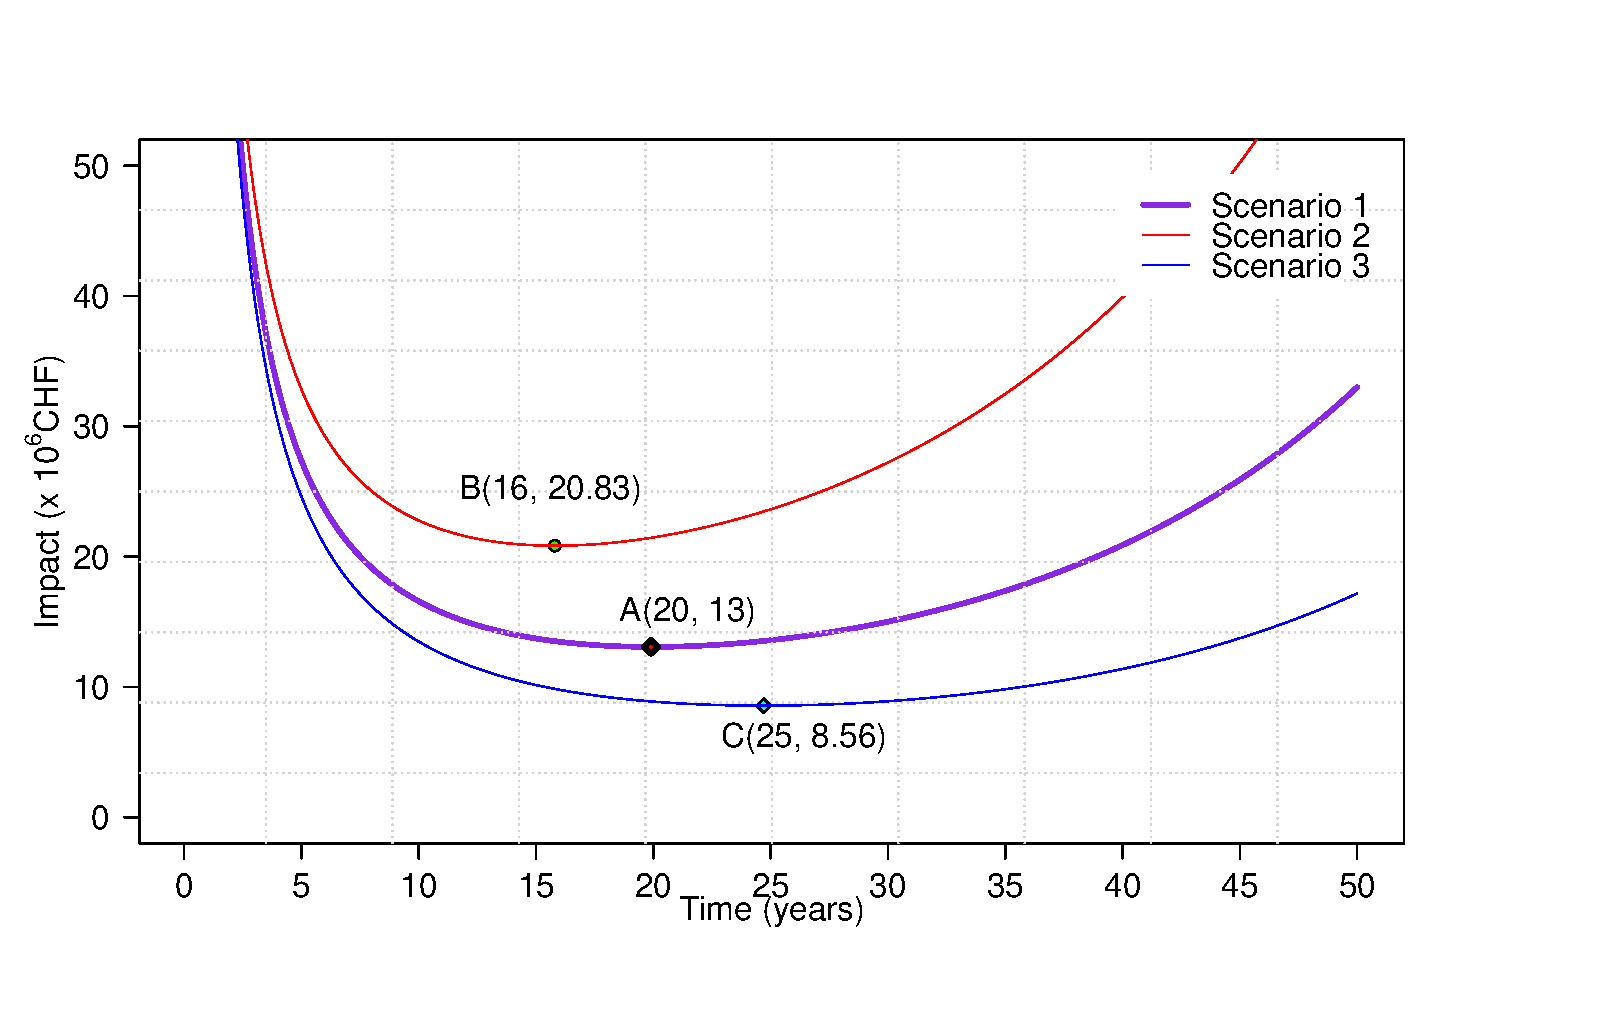
\includegraphics[scale=0.6]{fig2} 
\caption{Variogram of pavement indicators.} 
\label{fig2}
\end{figure}

Neither Fig. \ref{fig1} nor Fig. \ref{fig2} address the correlation across indicators. Table \ref{table2} shows that
coincident observations of different indicators are themselves correlated. This relationship provides a basis to predict 
one inspection type from the other. The potential usefulness is not limited to replacing one inspection type with 
another; additionally one obtains a second and third check on the plausibility of recorded observations that is in addition to 
the neighboring values of the same index. This also is a topic for further research.

\begin{table}
\begin{center}
\caption{Correlation across index types, common inspection year.}
\label{table2}
\begin{tabular}{c|cccc}\hline
\textbf{×} & I2-2004 & I2-2009 & I3-2004 & I3-2009\\\hline
I0-2004 & 0.29 & × & 0.28 & ×\\
I0-2009 & × & 0.18 & × & 0.09\\
I3-2004 & × & × & 0.17 & ×\\
I3-2009 & × & × & × & 0.35\\\hline
\end{tabular}
\end{center}
\end{table}

We now turn to how a univariate Kriging model can harness the spatial correlation of road serviceability indicators to 
predict values at a target location from observations at nearby locations.
%%%%
\section{The longitudinal univariate Kriging model} \label{krigmodel}
\subsection{General concept and model} \label{krigmodel1}
Kriging models have been extensively used in the field of geostatistics and others as well.
Various types of Kriging models exist \cite{Wackernagel1998}. The purpose of using the models
is to estimate the values of characteristic variables at one location, the estimation point, given
similar observations at surrounding locations, the data points. For instance, Kriging can be
used in environmental engineering to model how the degree of contamination of an unwanted
substance varies over a given area of land \cite{Cattle2002}.

In principle, Kriging is an interpolation based on a weighted average of surrounding data
points. The weights are a function of their spatial covariance values, which themselves are
assumed to be a function of distance. There are many good sources describing the actual
calculation of Kriging weights; e.g. \citeN{Wackernagel1998}, \citeN{Diggle2001}, and \citeN{Stein1999}
to which the interested reader is referred so that the discussion below may be kept to a
minimum. However, two basic effects are important to note. First, the closer a data point is to
an estimation point, the larger its weight in the estimation becomes. Second, the closer two
data points come to one another, the smaller the sum of their weights becomes, provided a
third data point exists to which the extra weight can be transferred. This is consistent with the
intuition that sampling twice at the same location does not add as much new information as
sampling twice at different locations would.

The selection of the data points for interpolation of a given estimation point, referred to as
clustering , plays an important role. Two counterbalancing forces are at work as will be shown
later in Fig. \ref{fig5} through Fig. \ref{fig7}. Theoretically, one can imagine that the wider a cluster
is, the more it includes points that have a small amount of predictive information. On the
other hand, the narrower the cluster, the fewer observations are available on which to base a
prediction. Thus, one question to address in Kriging is the selection of the cluster width. In
this paper we demonstrate an empirical approach to selecting the cluster width.

Some advantages of Kriging are that it:
\begin{itemize}
 \item Compensates for the effects of clustered data by assigning individual points within a
close proximity less weight than isolated data points and thereby treats clusters more like single
points;
\item Gives estimates of estimation errors (Kriging variance) in addition to the estimates of
the variables themselves;
\item Provides a basis for stochastic simulation of potential realizations through the
availability of estimation errors.
\end{itemize}
%%%
The following presentation follows \citeN{goovaerts1997}. Kriging estimators are variants of the basic linear regression estimator $Z^*(u)$ defined as 
%%
\begin{eqnarray}
&& Z^*(u)-m(u)=\sum_{\alpha=1}^{n(u)} \lambda_{\alpha} \left[ Z(u_{\alpha})-m(u_{\alpha}) \right],\label{zu}
\end{eqnarray}
%%
where,\\
%
\begin{tabular}{lp{13cm}}
$u,u_{\alpha}$: & Location vectors for the estimation point and one of the neighboring data points, indexed by 
$\alpha$\\
$n(u)$: & number of data points in a neighborhood that are used to estimate $Z^*(u)$\\
$m(u),m(u_{\alpha})$: & are the expected values of $Z(u)$ and $Z(u_{\alpha})$\\
$\lambda_{\alpha}(u)$: & Kriging weight assigned to data point $z(u_{\alpha})$ in the estimation of the estimation 
point $u$. Note, the same data point will receive a different weight if it is used to estimate a different estimation 
point.
\end{tabular}

$Z(u)$ is treated as a random field with its expected value, $m(u)$. The residual between the observed value and expected value is $R(u)=Z(u) - m(u)$. The objective of Kriging is to determine the weights, $\lambda_{\alpha}$, that minimize the variance of the estimator
%%
\begin{eqnarray}
&& \sigma_E^2(u)=Var\left[Z^*(u)-Z(u)\right],\label{detlta}
\end{eqnarray}
%%
under the unbiasedness constraint that
%%
\begin{eqnarray}
&& E\left\lbrace Z^*(u)-Z(u) \right\rbrace = 0  \label{zustart}
\end{eqnarray}
%%
After filtering out the trend, the residual random field $R(u)$ has a stationary mean of 0 and
a stationary covariance function, that is, covariance is a function of lag, $h$ , but not of
position, $u$ . Formally this is
%%
\begin{manyeqns}
&& E\left\lbrace R(u) \right\rbrace = 0  \label{covru} \\
&& Cov\left\lbrace R(u),R(u+h) \right\rbrace = E\left\lbrace R(u) R(u+h) \right\rbrace  \label{covru1}
\end{manyeqns}
%%
The covariance function is often derived in two steps as we do in this paper. First, the data is used to estimate a set 
of covariance observations for a discrete set of lag differences. \textcolor{red}{This step is done by using empirical semivariance function (\ref{semivariogramfun})
\begin{eqnarray}
&& \hat{\gamma}(h)=\frac{1}{2}\cdot \frac{1}{N(h)} \sum_{i=1}^{N(h)} \left ( Z(u_{\alpha}+h) - Z(u_{\alpha}) \right )^2  \label{semivariogramfun}
\end{eqnarray}
Where, $N(h)$ is number of pair data at distant $h$.} Next those estimates are fitted to a functional form to represent the variogram. These two steps are distinguished semantically as the ``empirical'' and the ``theoretical'' 
variagrams respectively. Examples of this process can be seen in Fig. \ref{fig4}. A typical form for the theoretical variogram
includes a so called ``nugget'' and ``sill''. The nugget is the discontinuous jump of the variogram at the origin where 
one is sampling at a distance of zero from one another. The sill is the upper bound of the covariance function where 
correlation between the observations has been reduced to zero.

There are three main variants of Kriging, simple, ordinary, and Kriging with a trend. They primarily differ in their 
treatments of the trend component, $m(u)$ . The interested reader is referred to the work of \citeN{goovaerts1997} and 
\citeN{Wackernagel1998}.
\subsection{Longitudinal structure of data} \label{krigmodel2}
In frequent practice, a road is divided first into directions and then into section-lanes of equal length $d$. 
Inspection data is acquired and stored for every triple: direction, section and lane. In our data, observations of 
highway pavement indicators are stored for each direction and every $100$ m length. No distinction is made for the lane 
so that we will refer only to road sections from here forward. The two directions of the road are treated as separate 
roads. Fig. \ref{fig3} illustrates the division of a road with many sections in both directions of traffic A and B. With 
incomplete inspection data, a value of one indicator $\bold x$ (e.g. cracking or roughness) of a section $s_n(n \in 1 \cdots 
N )$ would be absent in the database. However, the values for surrounding sections are available. The true value of 
$\bold x_n$ in section $s_n$ can be interpolated using a Kriging model and available data on $\bold x_{n\pm h}$ from nearby 
sections.

%
\begin{figure}
\centering
\includegraphics[scale=0.8]{fig3} 
\caption{Division of inspection data and clustering.} 
\label{fig3}
\end{figure}
%

As mentioned earlier, an important parameter of the model is the clustering distance $h^*$ . In
the context of estimating the value of $\bold x_n$ , clustering is the selection of sections within the
circular distance $h \le h^*$ of the targeted sections. For example, in Fig. \ref{fig3}, cluster 1 includes
two adjacent sections whereas cluster 2 includes four sections. We investigate below how the
predictive accuracy varies in the parameter $h^*$.
%%
\section{Estimation methodology} \label{krigestimate}
There is a rich literature describing \textcolor{red}{different algorithms to estimate the weights} for Kriging models \cite{Wackernagel1998}. \textcolor{red}{Since the estimating algorithms for Kriging models have well published, this work therefore employs a linear optimization algorithm developed in the R package ``GeoR'' \cite{Diggle2001,Diggle2007} and consider it as an internal part of the estimation methodology. The estimation methodology herein described in this section is thus not only about how to estimate the weights but about mainly on how to generate the test dataset from GIS database}. 

It is assumed that a structure of data that is commonly found in 
the database of a standard PMS. Table \ref{table3} depicts this structure. Let there be $R$ roads indexed by $r$ with each road  
divided into sections indexed by $n$. Data elements for a section include the position (e.g. coordinates, axis 
distance), the date and indicator values of different inspections as well as other attributes that may be stored for 
each section. This might include the date and type of previous interventions, characteristics of materials used, traffic volume, 
etc.


\begin{table}[htbp]
\begin{center}
\caption{Structure of the database}
\begin{tabular}{l|l|l|l|l|l|l|l|l|l|l|l}
\hline
\multicolumn{1}{c|}{Road} & \multicolumn{1}{c|}{Section} & \multicolumn{2}{c|}{Coordinates} & \multicolumn{4}{c|}{Inspection 1} & \multicolumn{4}{c}{Inspection 2} \\ 
\cline{3-12}
\multicolumn{1}{c|}{ID} & \multicolumn{1}{c|}{ID } & \multicolumn{1}{c|}{ X } & \multicolumn{1}{c|}{ Y } & \multicolumn{1}{c|}{Year } & \multicolumn{1}{c|}{ Ind. 1 } & \multicolumn{1}{c|}{ Ind. 2 } & \multicolumn{1}{c|}{ ... } & \multicolumn{1}{c|}{Year} & \multicolumn{1}{c|}{ Ind. 1 } & \multicolumn{1}{c|}{ Ind. 2 } & \multicolumn{1}{c}{ ... } \\ 
\hline
\multicolumn{1}{c|}{1} & \multicolumn{1}{c|}{1} & \multicolumn{1}{c|}{$x_1$} & \multicolumn{1}{c|}{$y_1$} & \multicolumn{1}{c|}{2008} & \multicolumn{1}{c|}{$v_1^1$} & \multicolumn{1}{c|}{$v_1^2$} & \multicolumn{1}{c|}{ ... } & \multicolumn{1}{c|}{2012} & \multicolumn{1}{c|}{ ... } & \multicolumn{1}{c|}{ ... } & \multicolumn{1}{c}{ ... } \\ 
\multicolumn{1}{c|}{1} & \multicolumn{1}{c|}{2} & \multicolumn{1}{c|}{$x_2$} & \multicolumn{1}{c|}{$y_2$} & \multicolumn{1}{c|}{2008} & \multicolumn{1}{c|}{$v_2^1$} & \multicolumn{1}{c|}{$v_2^2$} & \multicolumn{1}{c|}{ ... } & \multicolumn{1}{c|}{2012} & \multicolumn{1}{c|}{ ... } & \multicolumn{1}{c|}{ ... } & \multicolumn{1}{c}{ ... } \\ 
\multicolumn{1}{c|}{1} & \multicolumn{1}{c|}{3} & \multicolumn{1}{c|}{$x_3$} & \multicolumn{1}{c|}{$y_3$} & \multicolumn{1}{c|}{2008} & \multicolumn{1}{c|}{$v_3^1$} & \multicolumn{1}{c|}{$v_3^2$} & \multicolumn{1}{c|}{ ... } & \multicolumn{1}{c|}{2012} & \multicolumn{1}{c|}{ ... } & \multicolumn{1}{c|}{ ... } & \multicolumn{1}{c}{ ... } \\ 
\multicolumn{1}{c|}{2} & \multicolumn{1}{c|}{1} & \multicolumn{1}{c|}{ ... } & \multicolumn{1}{c|}{ ... } & \multicolumn{1}{c|}{2008} & \multicolumn{1}{c|}{ ... } & \multicolumn{1}{c|}{ ... } & \multicolumn{1}{c|}{ ... } & \multicolumn{1}{c|}{2012} & \multicolumn{1}{c|}{ ... } & \multicolumn{1}{c|}{ ... } & \multicolumn{1}{c}{ ... } \\ 
\multicolumn{1}{c|}{2} & \multicolumn{1}{c|}{2} & \multicolumn{1}{c|}{ ... } & \multicolumn{1}{c|}{ ... } & \multicolumn{1}{c|}{2008} & \multicolumn{1}{c|}{ ... } & \multicolumn{1}{c|}{ ... } & \multicolumn{1}{c|}{ ... } & \multicolumn{1}{c|}{2012} & \multicolumn{1}{c|}{ ... } & \multicolumn{1}{c|}{ ... } & \multicolumn{1}{c}{ ... } \\ 
\multicolumn{1}{c|}{2} & \multicolumn{1}{c|}{3} & \multicolumn{1}{c|}{ ... } & \multicolumn{1}{c|}{ ... } & \multicolumn{1}{c|}{2008} & \multicolumn{1}{c|}{ ... } & \multicolumn{1}{c|}{ ... } & \multicolumn{1}{c|}{ ... } & \multicolumn{1}{c|}{2012} & \multicolumn{1}{c|}{ ... } & \multicolumn{1}{c|}{ ... } & \multicolumn{1}{c}{ ... } \\ 
\multicolumn{1}{c|}{2} & \multicolumn{1}{c|}{4} & \multicolumn{1}{c|}{ ... } & \multicolumn{1}{c|}{ ... } & \multicolumn{1}{c|}{2008} & \multicolumn{1}{c|}{ ... } & \multicolumn{1}{c|}{ ... } & \multicolumn{1}{c|}{ ... } & \multicolumn{1}{c|}{2012} & \multicolumn{1}{c|}{ ... } & \multicolumn{1}{c|}{ ... } & \multicolumn{1}{c}{ ... } \\ 
\multicolumn{1}{c|}{...} & \multicolumn{1}{c|}{ ... } & \multicolumn{1}{c|}{ ... } & \multicolumn{1}{c|}{ ... } & \multicolumn{1}{c|}{2008} & \multicolumn{1}{c|}{ ... } & \multicolumn{1}{c|}{ ... } & \multicolumn{1}{c|}{ ... } & \multicolumn{1}{c|}{2012} & \multicolumn{1}{c|}{ ... } & \multicolumn{1}{c|}{ ... } & \multicolumn{1}{c}{ ... } \\ 
\multicolumn{1}{c|}{...} & \multicolumn{1}{c|}{ ... } & \multicolumn{1}{c|}{ ... } & \multicolumn{1}{c|}{ ... } & \multicolumn{1}{c|}{2008} & \multicolumn{1}{c|}{ ... } & \multicolumn{1}{c|}{ ... } & \multicolumn{1}{c|}{ ... } & \multicolumn{1}{c|}{2012} & \multicolumn{1}{c|}{ ... } & \multicolumn{1}{c|}{ ... } & \multicolumn{1}{c}{ ... } \\ 
\multicolumn{1}{c|}{R} & \multicolumn{1}{c|}{ ... } & \multicolumn{1}{c|}{ ... } & \multicolumn{1}{c|}{ ... } & \multicolumn{1}{c|}{2008} & \multicolumn{1}{c|}{ ... } & \multicolumn{1}{c|}{ ... } & \multicolumn{1}{c|}{ ... } & \multicolumn{1}{c|}{2012} & \multicolumn{1}{c|}{ ... } & \multicolumn{1}{c|}{ ... } & \multicolumn{1}{c}{ ... } \\ 
\hline
\end{tabular}
\label{table3}
\end{center}
\end{table}

One should think of each Kriged estimate for each specific point as if it were a separate
regression estimation. We therefore generate our test dataset by stepping through all the
potential target points and generating for each a Kriging estimate as if that observation were
missing. That process results in both an observed and predicted value for each road section in
the data set. The estimate itself requires selecting all the surrounding indicator values that are
contained within the cluster definition and feeding this data to the Kriging sub-routine which
returns the Kriging estimate for that point. One proceeds iteratively through all the estimation points as
follows:
%
\begin{itemize}
 \item Step 1: Select all road sections belonging to road $r$ ;
\item Step 2: Select the target section $(r,n)$. For example, select road $id=1$ and section $id=2$;
\item Step 3: Apply the cluster rule by selecting all points $(r,i)$ such that $Distance((r,n),(r,i))$ $\le h^*$. Each 
cluster can be assigned the index $(r,n)$ ;
\item Step 4: Call the Kriging procedure to estimate the value of the indicator at $(r,n)$ using the points in the cluster $(r,n)$ ;
\item Step 5: Return to Step 2 or Step 1 as the case may be until the estimation is complete for all road sections r and 
sections n .
\end{itemize}

\textcolor{red}{Since this methodology is used to generate test datasets from observed data and pretend the value at any target point as ``missing'', it is therefore not used for populating missing data in series. However, conceptually, if managers expect to estimate missing data in series, they can still use the Krigging models and develop a suitable algorithm to reestimate the missing data in series or they can combine the use of Krigging models with the SSA approach recommended by \citeN{AlZoubi2015}.} 

%
%An example of R code that implements the above steps is given in the Appendix for the application of Kriging. The code can be modified to suit the actual data structure.
\section{Case study} \label{casestudy}
\subsection{Overview of data} \label{casestudy1}
A case study was conducted on a dataset from the Swiss national highway system\footnote{We are grateful to the Swiss National Road Authority, ASTRA, for providing this data}. Inspection data was collected three 
times between the years 2000 to 2009. The observations were recorded by high speed inspection cars with one value 
recorded to represent the average state for each $100$ $m$ section. An overview of the number of observations is given in 
Table \ref{table4}. \textcolor{red}{This data set is considered as a complete set. This means there is no missing data. However, in the analysis, each observed value at any location will be treated as ``missing data'' and it is reestimated for the purpose of comparison with the observed one.}

\begin{table}[htbp]
\begin{center}
\caption{Data overview}
\begin{tabular}{l|p{6cm}|l|l|l}
\hline
\multicolumn{1}{c|}{I-values} &  Description  & \multicolumn{3}{c}{Numbers of data points} \\ 
\cline{3-5}
\multicolumn{1}{c|}{} &  & \multicolumn{1}{c|}{2000} & \multicolumn{1}{c|}{2004} & \multicolumn{1}{c}{2009} \\ 
\hline
\multicolumn{1}{c|}{I0} & Surface damage without consideration of rut index  & \multicolumn{1}{c|}{0} & \multicolumn{1}{c|}{28'983} & \multicolumn{1}{c}{35'022} \\ 
\multicolumn{1}{c|}{I2} & Longitudinal unevenness  & \multicolumn{1}{c|}{27'747} & \multicolumn{1}{c|}{29'046} & \multicolumn{1}{c}{35'330} \\ 
\multicolumn{1}{c|}{I3} & Transversal unevenness  & \multicolumn{1}{c|}{27'765} & \multicolumn{1}{c|}{29'131} & \multicolumn{1}{c}{35'339} \\ 
\hline
\end{tabular}
\label{table4}
\end{center}
\end{table}
%
\subsection{Design of cluster} \label{casestudy2}
As mentioned above, one of the parameters required in a Kriging routine is the definition of
clusters. In order to understand the impact of different definitions we calculated results for
two sets of cluster definitions and within each of these sets, we vary the circumference $h^*$. In
the first set, Scenario 1, all the available intermediate values were used. In the second set,
Scenario 2, we only use the two observations within the cluster that were furthest from the
target point. In this way, we simulate the effect that longer inspection intervals would have on
the Kriging estimates. In both scenarios, $h^*$ was varied in $100$ $m$ steps from $\pm 100$ $m$ to
$\pm 1000$ $m$.
\subsection{Generating a dataset of Kriged values} \label{casestudy3}
%%%
\subsubsection{Estimating the correlation function} \label{casestudy31}
Kriging begins with the estimation of a best fitting variogram $\hat \mu (h)$ from which a spatial
correlation function $\rho(h)$ can be extracted. The estimation involves first the selection of a
suitable functional form, and second, the estimation of best fitting parameters. Some general
functional forms for the correlation function are Cauchy, Circular, Cubic, Gaussian,
Exponential, Matern, and Spherical \cite{Wackernagel1998,Diggle2001}. In our
example, the exponential form in Eq. (\ref{muh}) was selected based on a visual examination of
the experimental variograms in Fig. \ref{fig2}. The basic fitting parameter is $\phi$ and $\beta_0$ represents the
nugget. It prevents the covariance from going to zero when $h$ is zero.
%%
\begin{eqnarray}
&& \mu(h)=2\sigma^2\left(1-\beta_0 exp(-\frac{h}{\phi})\right)  \label{muh}
\end{eqnarray}
%%
In log form, Eq. (\ref{muh}) can be estimated with OLS after minor rearrangement whereby $\mu(h)$ and $h$ are the sample 
covariance of indicator values and the interval distance respectively.

Using Eq. (\ref{varabh}), the functional form for the correlation function is then
\begin{eqnarray}
&& \rho(h)=\beta_0 exp(-\frac{h}{\phi})  \label{rhoh}
\end{eqnarray}
%%
\subsubsection{Calculating the covariance matrix for each cluster} \label{casestudy32}
The covariance matrix expresses the covariance between each point in the cluster and every other point in the cluster. 
Its role in Kriging is exactly the same as its role in a GLS regression. From the definition of covariance, and assuming 
variance is constant throughout the field, one may write the covariance function as
\begin{eqnarray}
&& C(h)=\sigma^2 \rho(h)  \label{Ch}
\end{eqnarray}

Cell $i$ , $j$ contains the value of this expression at the distance between points $i$ and $j$. The elements on the diagonal are all equal 
to the variance of the de-trended field.

The following figures (Fig. \ref{fig4}) show the theoretical variograms fitted to the sample variance of the difference in indicator 
values for each distance $h$ calculated for each of the values $I0$ , $I2$ , and $I3$ collected during the period 2000 to 2009. %The depicted relationships are used to krigg the values of each estimation point. One notes that each estimation point requires its own covariance matrix and yields its own set of optimal weights to apply to its set of data points.

\subsubsection{Calculating the predicted values} \label{casestudy33}
A predicted value of $I0$ , $I2$ , and $I3$ was generated for each inspection year and target point. The predicted 
values for each location are then compared to the observed values. Subtracting one from the other yields a residual (Fig. \ref{fig5} through Fig. \ref{fig7}). 
% It is possible to draw the density distribution for each cluster circumference $h^*$ from these residuals. Charts of the distributions can be seen in Fig. \ref{fig5} through Fig. \ref{fig12}. 
An interpretive discussion follows in the next section.
\subsection{Results} \label{casestudy4}
The results for each inspection index and year are summarized by density plots of the residuals as well as with curves showing the standard deviation and the mean of the residuals for each cluster concept and scenario in plots of Fig. \ref{fig5} through Fig. \ref{fig7}.

The goal of this research is to investigate the potential of Kriging as a methodology for predicting the serviceability indicators at locations where measurements are missing. The above figures suggest the following conclusion.
%
\subsubsection{Scenario 1: Clusters including intermediate observations} \label{casestudy41}
The predicted values show no particular bias. Relative to the size of the standard
deviations the mean residual values are very close to zero.

To consider how the distributions of the residuals change as the size of the clusters
$h^*$ increases, one must consult the results for Scenario 1. Looking at Fig. \ref{fig5} through
Fig. \ref{fig7} two general cases emerge. With $I0$ and $I3$ there is little change in the standard
deviation of the residuals as the cluster size changes. With $I2$ one can observe an
initial decline followed by a constant level. Table \ref{table5} shows the actual values. Local
minima are highlighted with bold print. From it one can see that values decline in all
cases except $I3$-2004, however the decline is very slight. Variation for $I1$ and $I3$ are within a range of 1\%. On the other hand, $I2$ declines visibly in all three years. The magnitude lies between 3\% and 5\%. Most of the variance reduction is achieved by a cluster size of $400$ $m$. For $I1$ and $I3$, clusters of size 100 $m$ seem equally effective as clusters of size 1000 $m$. One notes that estimates from a cluster size of $100$ $m$ is the simple average of the two nearest observation.

\begin{table}[htbp]
\begin{center}
\caption{Standard deviations of residuals, Scenario 1.}
\begin{tabular}{l|l|l|l|l|l|l|l|l}
\hline
\multicolumn{1}{c|}{Cluster} & \multicolumn{8}{c}{I values} \\ 
\cline{2-9}
\multicolumn{1}{c|}{boundary} & \multicolumn{2}{c|}{I0} & \multicolumn{3}{c|}{I2} & \multicolumn{3}{c}{I3} \\ 
\cline{2-9}
\multicolumn{1}{c|}{$h^*$} & \multicolumn{1}{c|}{2004} & \multicolumn{1}{c|}{2009} & \multicolumn{1}{c|}{2000} & \multicolumn{1}{c|}{2004} & \multicolumn{1}{c|}{2009} & \multicolumn{1}{c|}{2000} & \multicolumn{1}{c|}{2004} & \multicolumn{1}{c}{2009} \\ 
\hline
\multicolumn{1}{c|}{100} & \multicolumn{1}{c|}{0.07795} & \multicolumn{1}{c|}{0.14068} & \multicolumn{1}{c|}{0.29075} & \multicolumn{1}{c|}{0.21718} & \multicolumn{1}{c|}{0.54079} & \multicolumn{1}{c|}{0.21453} & \multicolumn{1}{c|}{\textbf{0.22456}} & \multicolumn{1}{c}{0.30764} \\ 
\multicolumn{1}{c|}{200} & \multicolumn{1}{c|}{0.07726} & \multicolumn{1}{c|}{0.13887} & \multicolumn{1}{c|}{0.28355} & \multicolumn{1}{c|}{0.21276} & \multicolumn{1}{c|}{0.52899} & \multicolumn{1}{c|}{0.21336} & \multicolumn{1}{c|}{0.22777} & \multicolumn{1}{c}{0.31044} \\ 
\multicolumn{1}{c|}{300} & \multicolumn{1}{c|}{0.07711} & \multicolumn{1}{c|}{0.13847} & \multicolumn{1}{c|}{0.2789} & \multicolumn{1}{c|}{0.21147} & \multicolumn{1}{c|}{0.51555} & \multicolumn{1}{c|}{0.21248} & \multicolumn{1}{c|}{0.22743} & \multicolumn{1}{c}{0.30682} \\ 
\multicolumn{1}{c|}{400} & \multicolumn{1}{c|}{0.07706} & \multicolumn{1}{c|}{0.13838} & \multicolumn{1}{c|}{0.27686} & \multicolumn{1}{c|}{0.21138} & \multicolumn{1}{c|}{0.5159} & \multicolumn{1}{c|}{0.21195} & \multicolumn{1}{c|}{0.22698} & \multicolumn{1}{c}{\textbf{0.30431}} \\ 
\multicolumn{1}{c|}{500} & \multicolumn{1}{c|}{\textbf{0.07705}} & \multicolumn{1}{c|}{\textbf{0.13837}} & \multicolumn{1}{c|}{0.27628} & \multicolumn{1}{c|}{0.21047} & \multicolumn{1}{c|}{0.5168} & \multicolumn{1}{c|}{0.21156} & \multicolumn{1}{c|}{0.22675} & \multicolumn{1}{c}{0.30557} \\ 
\multicolumn{1}{c|}{600} & \multicolumn{1}{c|}{0.07709} & \multicolumn{1}{c|}{0.1384} & \multicolumn{1}{c|}{\textbf{0.27542}} & \multicolumn{1}{c|}{0.20982} & \multicolumn{1}{c|}{0.51407} & \multicolumn{1}{c|}{\textbf{0.21146}} & \multicolumn{1}{c|}{0.22651} & \multicolumn{1}{c}{0.30469} \\ 
\multicolumn{1}{c|}{700} & \multicolumn{1}{c|}{0.07713} & \multicolumn{1}{c|}{0.13842} & \multicolumn{1}{c|}{0.27543} & \multicolumn{1}{c|}{0.21031} & \multicolumn{1}{c|}{0.51183} & \multicolumn{1}{c|}{0.2117} & \multicolumn{1}{c|}{0.22667} & \multicolumn{1}{c}{0.30612} \\ 
\multicolumn{1}{c|}{800} & \multicolumn{1}{c|}{0.07711} & \multicolumn{1}{c|}{0.13819} & \multicolumn{1}{c|}{0.27552} & \multicolumn{1}{c|}{0.20997} & \multicolumn{1}{c|}{0.51427} & \multicolumn{1}{c|}{0.21167} & \multicolumn{1}{c|}{0.22668} & \multicolumn{1}{c}{0.30704} \\ 
\multicolumn{1}{c|}{900} & \multicolumn{1}{c|}{0.07715} & \multicolumn{1}{c|}{0.13824} & \multicolumn{1}{c|}{0.27544} & \multicolumn{1}{c|}{\textbf{0.2096}} & \multicolumn{1}{c|}{0.51282} & \multicolumn{1}{c|}{0.21151} & \multicolumn{1}{c|}{0.22645} & \multicolumn{1}{c}{0.30671} \\ 
\multicolumn{1}{c|}{1000} & \multicolumn{1}{c|}{0.07716} & \multicolumn{1}{c|}{\textbf{0.13817}} & \multicolumn{1}{c|}{\textbf{0.27537}} & \multicolumn{1}{c|}{0.20997} & \multicolumn{1}{c|}{\textbf{0.51103}} & \multicolumn{1}{c|}{0.21146} & \multicolumn{1}{c|}{0.22656} & \multicolumn{1}{c}{0.30739} \\ 
\hline
\end{tabular}
\label{table5}
\end{center}
\end{table}


\begin{table}[htbp]
\begin{center}
\caption{Standard deviations of residuals, Scenario 2.}
\begin{tabular}{l|l|l|l|l|l|l|l|l}
\hline
\multicolumn{1}{c|}{Cluster} & \multicolumn{8}{c}{I values} \\ 
\cline{2-9}
\multicolumn{1}{c|}{boundary} & \multicolumn{2}{c|}{I0} & \multicolumn{3}{c|}{I2} & \multicolumn{3}{c}{I3} \\ 
\cline{2-9}
\multicolumn{1}{c|}{$h^*$} & \multicolumn{1}{c|}{2004} & \multicolumn{1}{c|}{2009} & \multicolumn{1}{c|}{2000} & \multicolumn{1}{c|}{2004} & \multicolumn{1}{c|}{2009} & \multicolumn{1}{c|}{2000} & \multicolumn{1}{c|}{2004} & \multicolumn{1}{c}{2009} \\ 
\hline
\multicolumn{1}{c|}{100} & \multicolumn{1}{c|}{\textbf{0.07795}} & \multicolumn{1}{c|}{\textbf{0.14068}} & \multicolumn{1}{c|}{\textbf{0.29075}} & \multicolumn{1}{c|}{\textbf{0.21718}} & \multicolumn{1}{c|}{\textbf{0.54079}} & \multicolumn{1}{c|}{\textbf{0.21453}} & \multicolumn{1}{c|}{\textbf{0.22456}} & \multicolumn{1}{c}{\textbf{0.30764}} \\ 
\multicolumn{1}{c|}{200} & \multicolumn{1}{c|}{0.09842} & \multicolumn{1}{c|}{0.19934} & \multicolumn{1}{c|}{0.33684} & \multicolumn{1}{c|}{0.26729} & \multicolumn{1}{c|}{0.58848} & \multicolumn{1}{c|}{0.26542} & \multicolumn{1}{c|}{0.29054} & \multicolumn{1}{c}{0.41459} \\ 
\multicolumn{1}{c|}{300} & \multicolumn{1}{c|}{0.10739} & \multicolumn{1}{c|}{0.22484} & \multicolumn{1}{c|}{0.34586} & \multicolumn{1}{c|}{0.29056} & \multicolumn{1}{c|}{0.57950} & \multicolumn{1}{c|}{0.28863} & \multicolumn{1}{c|}{0.32660} & \multicolumn{1}{c}{0.44583} \\ 
\multicolumn{1}{c|}{400} & \multicolumn{1}{c|}{0.11649} & \multicolumn{1}{c|}{0.23846} & \multicolumn{1}{c|}{0.34815} & \multicolumn{1}{c|}{0.29966} & \multicolumn{1}{c|}{0.64494} & \multicolumn{1}{c|}{0.30091} & \multicolumn{1}{c|}{0.34765} & \multicolumn{1}{c}{0.48296} \\ 
\multicolumn{1}{c|}{500} & \multicolumn{1}{c|}{0.12422} & \multicolumn{1}{c|}{0.25308} & \multicolumn{1}{c|}{0.35496} & \multicolumn{1}{c|}{0.29840} & \multicolumn{1}{c|}{0.66850} & \multicolumn{1}{c|}{0.31587} & \multicolumn{1}{c|}{0.37111} & \multicolumn{1}{c}{0.51858} \\ 
\multicolumn{1}{c|}{600} & \multicolumn{1}{c|}{0.13485} & \multicolumn{1}{c|}{0.26470} & \multicolumn{1}{c|}{0.35504} & \multicolumn{1}{c|}{0.30538} & \multicolumn{1}{c|}{0.66808} & \multicolumn{1}{c|}{0.33309} & \multicolumn{1}{c|}{0.39533} & \multicolumn{1}{c}{0.52315} \\ 
\multicolumn{1}{c|}{700} & \multicolumn{1}{c|}{0.14333} & \multicolumn{1}{c|}{0.27523} & \multicolumn{1}{c|}{0.36930} & \multicolumn{1}{c|}{0.31993} & \multicolumn{1}{c|}{0.67440} & \multicolumn{1}{c|}{0.35515} & \multicolumn{1}{c|}{0.42239} & \multicolumn{1}{c}{0.54351} \\ 
\multicolumn{1}{c|}{800} & \multicolumn{1}{c|}{0.15000} & \multicolumn{1}{c|}{0.28557} & \multicolumn{1}{c|}{0.38290} & \multicolumn{1}{c|}{0.32074} & \multicolumn{1}{c|}{0.68903} & \multicolumn{1}{c|}{0.36391} & \multicolumn{1}{c|}{0.43648} & \multicolumn{1}{c}{0.56676} \\ 
\multicolumn{1}{c|}{900} & \multicolumn{1}{c|}{0.16131} & \multicolumn{1}{c|}{0.29585} & \multicolumn{1}{c|}{0.38907} & \multicolumn{1}{c|}{0.32448} & \multicolumn{1}{c|}{0.67490} & \multicolumn{1}{c|}{0.36272} & \multicolumn{1}{c|}{0.43648} & \multicolumn{1}{c}{0.58576} \\ 
\multicolumn{1}{c|}{1000} & \multicolumn{1}{c|}{0.16908} & \multicolumn{1}{c|}{0.30255} & \multicolumn{1}{c|}{0.39459} & \multicolumn{1}{c|}{0.33652} & \multicolumn{1}{c|}{0.64653} & \multicolumn{1}{c|}{0.36843} & \multicolumn{1}{c|}{0.45262} & \multicolumn{1}{c}{0.60407} \\ 
\hline
\end{tabular}
\label{table6}
\end{center}
\end{table}
%
The distributions do not appear to be normal. This is confirmed by the Q-Q plots. Example of the Q-Q plots is given for $I0$ and shown in Fig. \ref{fig8}. One reason why normality cannot be expected is that residuals are confined to a bounded interval, this follows since the indicator values themselves are defined on an interval. The distributions have too much weight at the center to be normally distributed. This observation has implications for probabilistic statements, such as confidence intervals on the estimates which a researcher might wish to define for the Kriged estimates.

The magnitudes of the standard deviations of the residuals can most readily be
interpreted by comparing them to the magnitude of the range from which indicator
observations are drawn. More than 98\% of all observed indicator values in the data
set lie in the range 0 to 3 even if values up to 5 are in fact possible. Taking $[0, 3]$ as
the effective range of values, a standard deviation of 0.3 is then exactly 10\% of that
range. Only the standard deviations of $I2$-2009 is substantially above 0.3 having values
near 0.5. Whether or not this is considered a good prediction depends, of course, on
the application.

In many cases, noticeable differences exist between the standard deviations of
Kriging residuals for the same indicator across inspections. Compare for instance the
levels in Fig. \ref{fig6} for Scenario 1. Given our sample size of over 3'000
observations, sampling error seems an unlikely explanation. And, considering that the
physical processes determining spatial correlation are likely to be constant across
inspections, one can infer that the difference in predictive accuracy reflects the
consistency of the inspection process itself. It is hypothesized that a measure of
inspection accuracy can be built from a ratio of measured spatial correlation, therefore, we
leave this to future research.

\begin{figure}
     \begin{minipage}[h]{0.5\linewidth}
        \centering
        \includegraphics[scale=0.31]{expi02004}\\
				\footnotesize{(a)-I0-2004}
     \end{minipage}
\vspace{1.5mm}
    \begin{minipage}[h]{0.5\linewidth}
       \centering
       \includegraphics[scale=0.31]{expi02009}\\
			\footnotesize{(b)-I0-2009}
     \end{minipage}
\vspace{1.5mm}
    \begin{minipage}[h]{0.5\linewidth}
       \centering
       \includegraphics[scale=0.31]{expi22000}\\
			\footnotesize{(c)-I2-2000}
     \end{minipage}
\vspace{1.5mm}
    \begin{minipage}[h]{0.5\linewidth}
       \centering
       \includegraphics[scale=0.31]{expi22004}\\
			\footnotesize{(d)-I2-2004}
     \end{minipage}
\vspace{1.5mm}
    \begin{minipage}[h]{0.5\linewidth}
       \centering
       \includegraphics[scale=0.31]{expi22009}\\
			\footnotesize{(e)-I2-2009}
     \end{minipage}
\vspace{1.5mm}
    \begin{minipage}[h]{0.5\linewidth}
       \centering
       \includegraphics[scale=0.31]{expi32000}\\
			\footnotesize{(f)-I3-2000}
     \end{minipage}
\vspace{1.5mm}
    \begin{minipage}[h]{0.5\linewidth}
       \centering
       \includegraphics[scale=0.31]{expi32004}\\
			\footnotesize{(g)-I3-2004}
     \end{minipage}
\vspace{1.5mm}
    \begin{minipage}[h]{0.5\linewidth}
       \centering
       \includegraphics[scale=0.31]{expi32009}\\
			\footnotesize{(h)-I3-2009}
     \end{minipage}
		\caption{Variograms.}
\label{fig4}
\end{figure}
%%


\begin{figure}
     \begin{minipage}[h]{0.5\linewidth}
        \centering
        \includegraphics[scale=0.34]{residual-scn1-i02004.eps}
				\footnotesize{(a)-$Scenario$ 1-I0-2004}
     \end{minipage}
\vspace{3.00mm}
    \begin{minipage}[h]{0.5\linewidth}
       \centering
       \includegraphics[scale=0.34]{residual-scn2-i02004.eps}
			\footnotesize{(b)-$Scenario$ 2-I0-2004}
     \end{minipage}
\vspace{3.00mm}
    \begin{minipage}[h]{0.5\linewidth}
       \centering
       \includegraphics[scale=0.34]{residual-scn1-i02009.eps}
			\footnotesize{(c)-$Scenario$ 1-I0-2009}
     \end{minipage}
\vspace{3.00mm}
    \begin{minipage}[h]{0.5\linewidth}
       \centering
       \includegraphics[scale=0.34]{residual-scn2-i02009.eps}
			\footnotesize{(d)-$Scenario$ 2-I0-2009}
     \end{minipage}
		\caption{Residuals-I0.}
\label{fig5}
\end{figure}
%%

\begin{figure}
 \begin{minipage}[h]{0.5\linewidth}
        \centering
        \includegraphics[scale=0.34]{residual-scn1-i22000.eps}
				\footnotesize{(a)-$Scenario$ 1-I2-2000}
     \end{minipage}
\vspace{3.00mm}
    \begin{minipage}[h]{0.5\linewidth}
       \centering
       \includegraphics[scale=0.34]{residual-scn2-i22000.eps}
			\footnotesize{(b)-$Scenario$ 2-I2-2000}
     \end{minipage}
\vspace{3.00mm} 
    \begin{minipage}[h]{0.5\linewidth}
        \centering
        \includegraphics[scale=0.34]{residual-scn1-i22004.eps}
				\footnotesize{(c)-$Scenario$ 1-I2-2004}
     \end{minipage}
\vspace{3.00mm}
    \begin{minipage}[h]{0.5\linewidth}
       \centering
       \includegraphics[scale=0.34]{residual-scn2-i22004.eps}
			\footnotesize{(d)-$Scenario$ 2-I2-2004}
     \end{minipage}
\vspace{3.00mm}
    \begin{minipage}[h]{0.5\linewidth}
       \centering
       \includegraphics[scale=0.34]{residual-scn1-i22009.eps}
			\footnotesize{(e)-$Scenario$ 1-I2-2009}
     \end{minipage}
\vspace{3.00mm}
    \begin{minipage}[h]{0.5\linewidth}
       \centering
       \includegraphics[scale=0.34]{residual-scn2-i22009.eps}
			\footnotesize{(f)-$Scenario$ 2-I2-2009}
     \end{minipage}
		\caption{Residuals-I2.}
\label{fig6}
\end{figure}

\begin{figure}
 \begin{minipage}[h]{0.5\linewidth}
        \centering
        \includegraphics[scale=0.34]{residual-scn1-i32000.eps}
				\footnotesize{(a)-$Scenario$ 1-I3-2000}
     \end{minipage}
\vspace{3.00mm}
    \begin{minipage}[h]{0.5\linewidth}
       \centering
       \includegraphics[scale=0.34]{residual-scn2-i32000.eps}
			\footnotesize{(b)-$Scenario$ 2-I3-2000}
     \end{minipage}
\vspace{3.00mm} 
    \begin{minipage}[h]{0.5\linewidth}
        \centering
        \includegraphics[scale=0.34]{residual-scn1-i32004.eps}
				\footnotesize{(c)-$Scenario$ 1-I3-2004}
     \end{minipage}
\vspace{3.00mm}
    \begin{minipage}[h]{0.5\linewidth}
       \centering
       \includegraphics[scale=0.34]{residual-scn2-i32004.eps}
			\footnotesize{(d)-$Scenario$ 2-I3-2004}
     \end{minipage}
\vspace{3.00mm}
    \begin{minipage}[h]{0.5\linewidth}
       \centering
       \includegraphics[scale=0.34]{residual-scn1-i32009.eps}
			\footnotesize{(e)-$Scenario$ 1-I3-2009}
     \end{minipage}
\vspace{3.00mm}
    \begin{minipage}[h]{0.5\linewidth}
       \centering
       \includegraphics[scale=0.34]{residual-scn2-i32009.eps}
			\footnotesize{(f)-$Scenario$ 2-I3-2009}
     \end{minipage}
		\caption{Residuals-I3.}
\label{fig7}
\end{figure}

\begin{figure}
     \begin{minipage}[h]{0.5\linewidth}
        \centering
        \includegraphics[scale=0.34]{qqd400scn1I02004.eps}
				\footnotesize{(a)-$Scenario$ 1-I0-2004}
     \end{minipage}
\vspace{5.00mm}
    \begin{minipage}[h]{0.5\linewidth}
       \centering
       \includegraphics[scale=0.34]{qqd400scn2I02004.eps}
			\footnotesize{(b)-$Scenario$ 2-I0-2004}
     \end{minipage}
\vspace{5.00mm}
    \begin{minipage}[h]{0.5\linewidth}
       \centering
       \includegraphics[scale=0.34]{qqd400scn1I02009.eps}
			\footnotesize{(c)-$Scenario$ 1-I0-2009}
     \end{minipage}
\vspace{3.00mm}
    \begin{minipage}[h]{0.5\linewidth}
       \centering
       \includegraphics[scale=0.34]{qqd400scn2I02009.eps}
			\footnotesize{(d)-$Scenario$ 2-I0-2009}
     \end{minipage}
		\caption{Normal Q-Q plot at distance d=400m-I0 value.}
\label{fig8}
\end{figure}
%%
%%

%
%\begin{figure}
%\centering
%\includegraphics[scale=0.8]{density} 
%\caption{Probability density.} 
%\label{fig16}
%\end{figure}
%

%
%\begin{figure}
%\centering
%\includegraphics[scale=0.8]{cdf} 
%\caption{Cummulative density function.} 
%\label{fig17}
%\end{figure}
%
\subsubsection{Scenario 2: including only the boundary data points} \label{casestudy42}
As can be seen by the blue triangle line in Fig. \ref{fig5} through Fig. \ref{fig7} for each data set, the standard deviation of the residual is 
increasing as the cluster size is expanding. This is not surprising since all intermediate values are being dropped. The increasing standard deviation reflects the loss of correlation between to measurements as the distance between them increases. The standard deviation of the residual increases by between 50\% and 100\% in all cases when the inspection interval distance is increased from $100$ $m$ to $1000$ $m$. A degree of non-linearity is apparent. This must be so since the sample variance over all values is an upper bound on the covariance.

The means of the residuals are largely unaffected by the distance between included observations which confirms the 
unbiasedness of the estimation procedure.

In absence of information on the cost and benefit of an additional inspection observation to calculate a loss function, nothing definite can be said about the optimal inspection interval. Nevertheless, a basis for considering the calculation is definitely present in the clear evidence of spatial correlation.

In order to answer the question as to which cluster length results in the lowest variance, Table \ref{table5} and Table \ref{table6} list the observed standard deviations of the residuals for each cluster concept and scenario. Values in bold are local minima.
\subsubsection{A measure of predictive accuracy} \label{casestudy43}
A measure of the predictive accuracy can be built by comparing the sum of squared residuals
to the total sum of squares as in the $R2$ of a standard regression. The values shown in Table \ref{table7}
are calculated using that cluster concept that resulted in the minimum variance of the
residuals. Only values for Scenario 1 are shown. The interpretation is the same as it would be
for any regression. An $R2$ of 90\% certainly confirms the viability of Kriging as a means of
filling in missing values for $I1$, but this level of predictive accuracy is dependent on the length
of the inspection interval, which in this case is 100 $m$. The explained variance with respect to
$I3$ is not quite as good, but it is still above 80\%. The $R2$ values for $I2$ are inconsistent,
particularly for 2009 ranging from a low of 39\% to a high of 66\%. Both the goodness of fit of
the variogram as well as degree of spatial correlation contribute to the $R2$. In the case of
$I2$-2009 the low result cannot be explained by a lower spatial correlation as can be seen in Fig. \ref{fig2}, but the fit of the variogram shown in Fig. \ref{fig4} does seem less tight than either $I2$-2000 or
$I2$-2004.

\begin{table}[htbp]
\begin{center}
\caption{Variance ratio (scenario 1).}
\begin{tabular}{l|l|l|l|l}
\hline
\multicolumn{1}{c|}{Indicators} & \multicolumn{1}{c|}{Population variance  of Indices} & \multicolumn{1}{c|}{Min residual variance} & \multicolumn{1}{c|}{$r2$} & \multicolumn{1}{c}{Cluster} \\ 
\cline{2-4}
\multicolumn{1}{c|}{(in year)} & \multicolumn{1}{c|}{(a)} & \multicolumn{1}{c|}{(b)} & \multicolumn{1}{c|}{1-(b/a)} & \multicolumn{1}{c}{boundary $h^*$} \\ 
\hline
\multicolumn{1}{c|}{I0-2004} & \multicolumn{1}{c|}{0.073} & \multicolumn{1}{c|}{0.006} & \multicolumn{1}{c|}{0.919} & \multicolumn{1}{c}{500} \\ 
\multicolumn{1}{c|}{I0-2009} & \multicolumn{1}{c|}{0.184} & \multicolumn{1}{c|}{0.019} & \multicolumn{1}{c|}{0.896} & \multicolumn{1}{c}{1000} \\ 
\multicolumn{1}{c|}{I2-2000} & \multicolumn{1}{c|}{0.413} & \multicolumn{1}{c|}{0.176} & \multicolumn{1}{c|}{0.575} & \multicolumn{1}{c}{800} \\ 
\multicolumn{1}{c|}{I2-2004} & \multicolumn{1}{c|}{0.201} & \multicolumn{1}{c|}{0.068} & \multicolumn{1}{c|}{0.663} & \multicolumn{1}{c}{600} \\ 
\multicolumn{1}{c|}{I2-2009} & \multicolumn{1}{c|}{0.419} & \multicolumn{1}{c|}{0.255} & \multicolumn{1}{c|}{0.391} & \multicolumn{1}{c}{900} \\ 
\multicolumn{1}{c|}{I3-2000} & \multicolumn{1}{c|}{0.242} & \multicolumn{1}{c|}{0.045} & \multicolumn{1}{c|}{0.815} & \multicolumn{1}{c}{600} \\ 
\multicolumn{1}{c|}{I3-2004} & \multicolumn{1}{c|}{0.316} & \multicolumn{1}{c|}{0.050} & \multicolumn{1}{c|}{0.841} & \multicolumn{1}{c}{100} \\ 
\multicolumn{1}{c|}{I3-2009} & \multicolumn{1}{c|}{0.412} & \multicolumn{1}{c|}{0.093} & \multicolumn{1}{c|}{0.775} & \multicolumn{1}{c}{400} \\ 
\hline
\end{tabular}
\label{table7}
\end{center}
\end{table}

\section{Conclusion}\label{conclusion}
This paper presents a methodology to predict the value of pavement indicators of a road
section using a Kriging model, which is widely used in geostatistics. It has been shown
through variograms that the preconditions for predictions are present but that these vary in
detail depending on the indicator, that is, the road characteristic of interest. It follows that the
optimal method of predicting will vary by road characteristic as well.

The proposed methodology has two important practical applications: 1) when there are
missing or questionable records of pavement indicators in the data inventory of the pavement
management system and 2) when an inspection value is needed at a point where none was
taken. Later instances are the norm rather than the exception when inspection data is
combined with other GIS information elements that use a different set of boundaries to
describe the spatial data.

The methodology was tested and confirmed on a dataset from the Swiss national highway
system. \textcolor{red}{It can be concluded from the example that there exists certain levels of spatial correlation on the value of serviceability indicators (e.g. within a distance of 400 m). This spatial correlation can be considered as a managerial indicator that can help managers to decide on dealing with missing data and on formulating possible future inspection strategies.} However, this paper is limited to only one specific kind of Kriging model. Numerous
extensions and variations are possible. Of particular interest is a multivariate Kriging approach that estimates values 
of one pavement indicator using values of itself and other
pavement indicators. A practical use would be to predict the bearing capacity of road
structures, which is normally done by the expensive Falling Weight Deflectometer (FWD)
method. One can make use of other indicators such as cracking and roughness to predict the
value of FWD and potentially reduce the inspection cost. A study on multivariate Kriging
models using the same set of data will be a topic of future research.

%
\pagebreak
%
%
% Now we start the appendices, with the new section name, "Appendix", and a 
%  new counter, "I", "II", etc.
%
\appendix\label{section:references}
%
% Here's the first appendix, the list of references:
%
\bibliography{ascexmpl}
%
% And now for some pretty impressive notation.  In this example, I have used
%   the tabular environment to line up the columns in ASCE style.
%   Note that this and all appendices (except the references) start with 
%   the \section command
%
\appendix\label{section:R Code}

%
\end{document}
